\documentclass[12pt,a4paper]{report}
\usepackage[T1]{fontenc}
\usepackage[english]{babel}
\usepackage[latin1]{inputenc} % per mettere le lettere accentate
%\usepackage[latin1]{inputenc}



   %%%%%%%%%%%%%%%%%%%%%%%%%%%%%%%%%%%%%%%%%%%%%%%%%%%%%%%%%
\usepackage{frontespizio}
% Col pacchetto tocbibind compariranno nell'indice anche
% la bibliografia ed eventualmente l'indice analitico
\usepackage[nottoc]{tocbibind}

% Il pacchetto indentfirst abolisce la fastidiosa convenzione
% anglosassone di fa cominciare la prima riga di un
% capitolo o sezione a margine sinistro, senza rientro:
\usepackage{indentfirst}

%\usepackage{graphicx} % gia' caricato da uniudtesi
%\graphicspath{{./figure/}}
%\usepackage{epstopdf}

 %%%%%%%%%%%%%%%%%%%%%%%%%%%%%%%%%%%%%%%%%%%%%%%%

\usepackage{amsmath,amsfonts,amssymb,amsthm}
\usepackage{latexsym}
\usepackage{mathtools}


%%%%%%%%%%%%%%%%%%%%%%%%%%%%%%%%%%%%%%%%%%%%%%%%%%%%%%%


   %%%%%%%%%%%%%%%%%%%%%%%%%%%%%%%%%%%%%%%%%%%

\newcommand{\N}{\mathbb{N}}
\newcommand{\Z}{\mathbb{Z}}
\newcommand{\K}{\mathbb{K}}
\newcommand{\R}{\mathbb{R}}
\newcommand{\C}{\mathbb{C}}
\newcommand{\V}{\mathcal{V}_{t}}
\newcommand{\mS}{\mathcal{S}_{t}}
\newcommand{\Div}{\text{div}}
\newcommand{\I}{\mathbb{I}}

   %%%%%%%%%%%%%%%%%%%%%%%%%%%%%%%%%%%%%%%%%%%%

\DeclareMathOperator{\traccia}{tr}
\DeclareMathOperator{\sen}{sen}
\DeclareMathOperator{\cl}{cl}
\DeclareMathOperator{\dom}{dom}
\DeclareMathOperator{\dist}{dist}
\DeclareMathOperator{\arcsen}{arcsen}
\DeclareMathOperator*{\maxlim}{max\,lim}
\DeclareMathOperator*{\minlim}{min\,lim}
\DeclareMathOperator*{\deepinf}{\phantom{\makebox[0pt]{p}}inf}

\DeclarePairedDelimiter{\norm}{\lVert}{\rVert}
    %%%%%%%%%%%%%%%%%%%%%%%%%%%%%%%%%%%%%%%%%%%%

\newcommand{\varsum}[3]{\sum_{#2}^{#3}\!
   {\vphantom{\sum}}_{#1}\;}
\newcommand{\varprod}[3]{\sum_{#2}^{#3}\!
   {\vphantom{\sum}}_{#1}\;}
\newcommand{\abs}[1]{\lvert#1\rvert} %Mi permette di fare il valore assoluto con un semplice comando
\newcommand{\opnorm}[1]{% 
  \left\vert\mkern-1mu\left\vert\mkern-1mu\left\vert #1 
    \right\vert\mkern-1mut\right\vert\mkern-1mu\right\vert}

\newcommand{\mnorm}[1]{% 
  \left\vert\mkern-1mu\left\vert\mkern-1mu\left\vert #1 
    \right\vert\mkern-1mu\right\vert\mkern-1mu\right\vert}


%%%************************************** Commento di marco: ho commentato questa parte perchè mi dava errore nella compilazione
\theoremstyle{plain}
\newtheorem{theorem}{Theorem}[chapter]
\newtheorem{proposition}[theorem]{Proposition}
\newtheorem{lemma}[theorem]{Lemma}
\newtheorem{corollary}[theorem]{Corollary}
\newtheorem{hypothesis}[theorem]{Hypothesis}

\theoremstyle{definition}
\newtheorem{definition}[theorem]{Definition}
\newtheorem{example}[theorem]{Example}
%
\theoremstyle{remark}
\newtheorem{observation}{Observation}[chapter]


%\usepackage{enumerate}
%*******************************************************
  
 \begin{document}
\title{\textbf{Perfect Matching}} %Review
\author{Marco Daresta, Chiara Langella, \\ Elisa Pontiroli and Alessandro Zeggiotti }
\date{2017-2018}
\maketitle
\chapter*{Abstract}
Graph theory has a precise date of birth: 1736. On that date, the Swiss mathematician Leonhard Euler solved the problem known as the seven bridges of K�nigsberg. One wondered if it was possible to take a walk in the city, to leave and arrive at the same point, so as to cross all the bridges exactly once.

Subsequently, in 1859 Hamilton proposed a game that, in several aspects, was linked to his theory of quaternions: the game of the icosahedron (which was actually played on a dodecahedron) was as follows: Hamilton had assigned to each vertex the name of a city and required to find a path that went around the world, that is to visit all the cities only once, and then return to the starting point.

A variant of the icosahedron game is the traveling salesman problem (TSP). It is a question of finding the shortest closed path in a complete weighed graph, ie the sides of which have different lengths.
This is the problem par excellence in combinatorial optimization.

It is not a problem to find a closed loop: in a complete graph at $n$ nodes there exists $ \frac{1}{2}(n-1)! $ closed circuits.
The problem is finding the best one.

Finding an algorithm that can solve every example of TSP would be an important change of horizon in mathematics: using this method, we would be able to efficiently solve every computational problem for which the answer is easily verifiable. Many consider it impossible.

In particular, in mathematics, computer science and, precisely, combinatorial geometry, graph theory deals with the study of graphs, which are discrete objects that make it possible to schematize a great variety of situations and processes and often allow analysis in quantitative terms and algorithms.

By graph we mean a structure consisting of:
\begin {itemize}
\item simple objects, called vertices or nodes;
\item links between vertices; these links can be:
\begin {itemize}
\item not oriented (ie with a direction, but not with a direction): in this case they are called edges, and the graph is called "not oriented";
\item oriented (ie with a direction and a verse): in this case they are called arcs or paths, and the graph is called "oriented" or digraph;
\item any data associated with nodes and / or links; a weighted graph is an example of a graph in which a numerical value, called "weight", is associated with each link.
\end {itemize}
\end {itemize}

A graph is generally represented on the plane by points or circles, which represent the nodes; the connections between the vertices are represented by segments or curves that connect two nodes; while, in the case of an oriented graph, the direction of the arcs is indicated by an arrow.
The same graph can be drawn in many different ways without changing its properties.

The structures that can be represented by graphs are present in many disciplines and many problems of practical interest can be formulated as graph-related issues. In particular, networks can be described in the form of graphs.
Oriented graphs are also used to represent finite state machines and many other formalisms, such as flowcharts, Markov chains, entity-relationship schemas and Petri nets.

The development of algorithms for manipulating graphs is one of the areas of greatest interest in information technology.

As part of the Operational Research, it is to be solved problems of minimum (and vice versa maximum) under appropriate restrictions imposed by the problem under examination and with particular methods that are still being studied. However, it almost always talk about optimizing a rather complex problem. The algorithms created for the resolution of seemingly insoluble problems are the backbone of all the Operations Research and simple reasoning can be thought of by powerful computers to solve problems with hundreds or thousands of variables.

Returning, however, to analyze the theory of the Graphs, unlike many other branches of Operations Research, this work certainly under the graphical display of arcs, nodes and streams. It is noted that any problem of Graphs and Networks apparently describable only in graphical form, instead has its own possible mathematical description and in particular, a linear, linear or non-linear programming formulation.

In this paper we will discuss in particular, after a brief introductory chapter on the graphs and the problem of Perfect Matching, aimed at clarifying definitions and theorems for a greater understanding and a general view of the problem, an algorithm for solving the problem of the Perfect Matching using both the Gurobi and Python languages, related by some examples.



\tableofcontents
\chapter{Introduction to the Problem of Perfect Matching}
Graph Theory is a branch of Mathematics and Computer Science whose goal is the study of graphs. These ones are objects which allows to schematize situations, processes in order to analize them in quantitative and algorithmic terms. They are also object of study mainly in Computer Science thanks to the development of specific algorithms. In graph theory there are a lot of problems: one of the most famous is about the Perfect Matching. Before we introduce it, we are going to recall some useful definition, notions and results.

% 1.1
\section{Some Generalities about Graphs}
\begin{definition}
We define $graph$ a ordered pair $G$ $=$ $(V,E)$ comprising a set V of vertices (or nodes) together with a set E of edges (or arcs) which are 2-element subsets of V.\\
\\
Given a graph G, with |V(G)| we denote the order of G, i.e the number of vertices of G while with |E(G)| we denote the size of G, i.e the number of edges of G\\
\\
A vertex $v \in V$ is incident to an edge $e \in E$ se $v \in e$.\\
Two edges $e_{1}, e_{2} \in E$ are incident (or adjacent) if they are a common vertex.\\
Two vertices $v_{1}, v_{2} \in V$ are adjacent if there exist an edge e $\in E$ such that $e=v_{1}v_{2}$.
\end{definition}

\begin{definition}
Let $G$ $=$ $(V,E)$ e $G'$ $=$ $(V',E')$ be two graphs. If $V'\subseteq V$ and $E'\subseteq E$, then $G'$ is a subgraph of $G$.
Moreover, if $G\ne G$, then we say that $G'$ is a proper subgraph of $G$.
\end{definition}

\begin{definition}
Let $G$ $=$ $(V,E)$ be a graph and let $v \in V$ be a vertex. The degree of a vertex $v$ is defined as
\begin{equation*}
d_{G}(V) := |N_{G}(v)|
\end{equation*}
where $N_{G}(v) := \left \{ w \in V : vw \in E \right \}$ is the neighbour of v. In other words, it is the number of edges incident to the vertex $v \in V$.
Next, we define
\begin{equation*}
\delta(G) := \min\limits_{v \in V} d_{G}(v) \in \mathbb{Z}
\end{equation*}
the minimum degree of G, i.e. the degree of the vertex of less incident edges and
\begin{equation*}
\Delta(G) := \max\limits_{v \in V} d_{G}(v) \in \mathbb{Z}
\end{equation*}
the maximum degree of G, i.e. the degree of the vertex with more incident edges.
Furthermore, we denote the average degree of G as
\begin{equation*}
d(G) := \frac{1}{|V|} \sum_{v \in V} d_{G}(v)
\end{equation*}
Obviously, we have that $\delta(G) \le d(G) \le \Delta(G)$.
\end{definition}

\begin{definition}
A graph $G$ $=$ $(V,E)$ is said to be K-regular if 
\begin{equation*}
d_{G} = k \qquad \forall v \in V
\end{equation*}
In other words, if all vertices have the same degree. As a consequence, we have $\delta = d = \Delta$.
In particular, 3-regular graphs are called also cubic graphs.
\end{definition}

\begin{definition}
A path is a graph $P = (V,E)$ on the form $V = \left \{x_{0}x_{1}, x_{1}x_{2}, \dots, x_{k-1}x_{k} \right \}$ where\\
$x_{0}$ e $x_{k}$ are called ends of P;\\
$x_{2}, \dots, x_{k-1}$ are the inner vertices of P;\\
The number of edges is the length of P;\\ 
With $P_{k}$ we mean a path of lenght $k$.
\end{definition}

\begin{definition}
A graph is said to be complete if every vertex is linked to all remaining vertices . It is denoted with $K_{n}$ (with $n \in N $ the number of vertices)
\end{definition}

\begin{definition}
A graph $G$ $=$ $(V,E)$ is bipartite if its vertex set $V$ can be partitioned into two disjoint subsets $V$ $=$ $V_{1} \cup V_{2}$ such that every edge $e \in E$ has the form $v_{1}v_{2}$, with $v_{1} \in V_{1}$ and $v_{2} \in V_{2}$.
\end{definition}

\begin{definition}
We define a planar graph $G$ a graph such that it can be rapresented  in a plane in order that they do not admite edges who intersect each other.\\
The complete graphs $K_{5}$ e $K_{3,3}$ are non-planar graphs.
\end{definition}
We report some example:

\begin{figure}[htbp]
\begin{minipage}[htbp]{.50\textwidth}
\centering
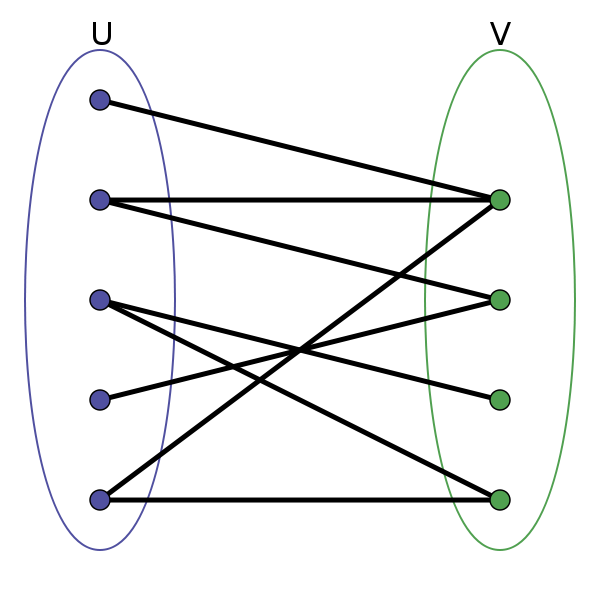
\includegraphics[width=.60\textwidth]{bipartito.png}
\caption{Bipartite graph}
\end{minipage}
\begin{minipage}[htbp]{.50\textwidth}
\centering
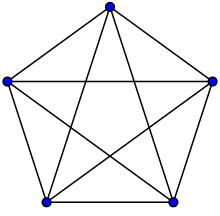
\includegraphics[width=.60\textwidth]{K5.png}
\caption{Complete graph ($K_{5}$)}
\end{minipage}
\medskip
\begin{minipage}[htbp]{.50\textwidth}
\centering
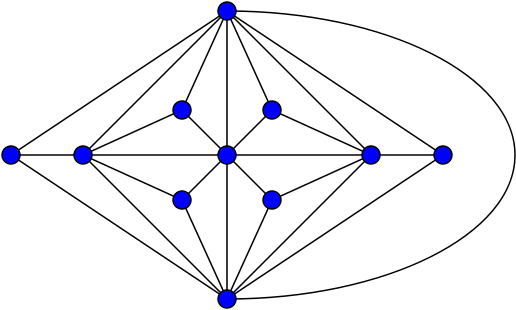
\includegraphics[width=.60\textwidth]{planare.png}
\caption{Planar graph}
\end{minipage}
\end{figure}
%1.2
\section{Matching and Perfect Matching}
Given a graph G, we want to find as many incident edges as possible.

\begin{definition}
Given a graph $G = (V,E)$, a matching $M(G)$ in $G$ is a set of pairwise non-adjacent edges; that is, no two edges share a common vertex. Or, in an equivalent form, if every vertex of G is incident to at most an edge in M, i.e. $deg(v)<= 1 \forall v\in G$.\\
This means that, in a matching M(G), all vertices can have either degree 0 or 1. In particular
\begin{itemize}
\item se deg(v) = 1, then the vertex v is matched (or saturated) if it is an endpoint of one of the edges in the matching.
\item se deg(v) = 0, then the vertex v is unmatched.
\end{itemize}
In a matching, two edges cannot be incident: if they were, then the vertex incident to these two edges would have degree 2, but this is not possible by definition.
\end{definition}

\begin{figure}[htbp]
\centering
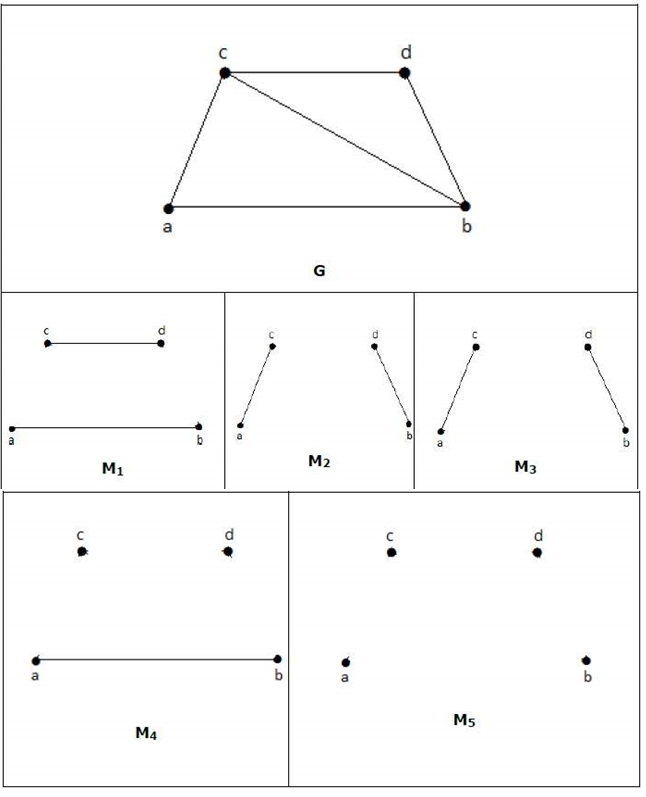
\includegraphics[width=.55\textwidth]{matching.png}
\caption{Examples of Matching of a graph G}
\end{figure}

\begin{definition}
Given $G = (V,E)$, a maximal matching is a matching M of a graph G with the property that if any edge not in M is added to M, it is no longer a matching, that is, M is maximal if it is not a subset of any other matching in graph G
\end{definition}

\begin{figure}[htbp]
\centering
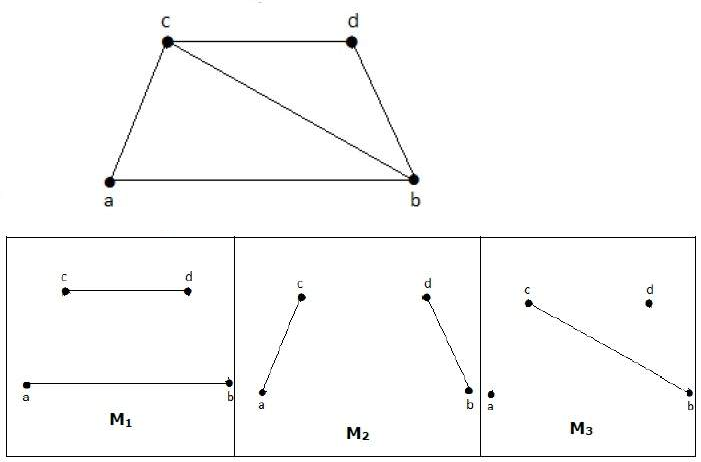
\includegraphics[width=.60\textwidth]{maximal.png}
\caption{$M_{1},M_{2},M_{3}$ are maximal matching for G}
\end{figure}

\begin{definition}
A maximum matching M(G) is a matching that contains the largest possible number of edges. There may be many maximum matchings and such number is called matching number. Note that every maximum matching is maximal, but not every maximal matching is a maximum matching. The following figure shows examples of maximum matchings in the same three graphs.
\end{definition}

\begin{figure}[htbp]
\centering
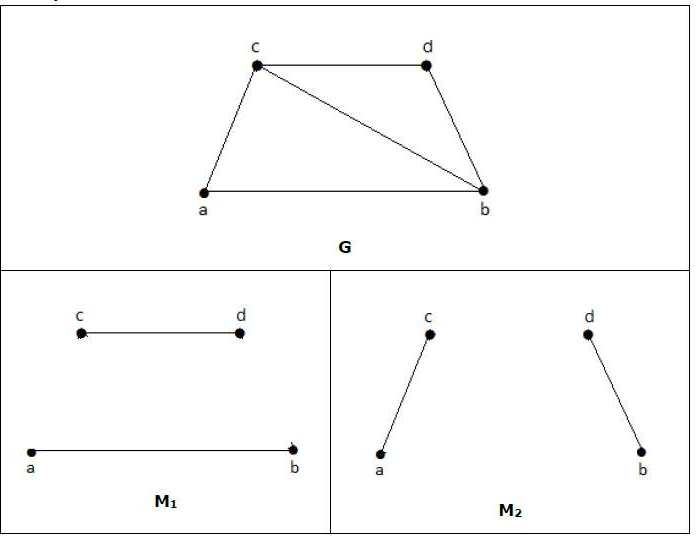
\includegraphics[width=.60\textwidth]{maximum.png}
\caption{$M_{1}$ e $M_{2}$ are maximum matching for G and the matching number is 2. Hence, using the graph G, we can form only subgraphs with at most 2 edges. For this reason we have 2 as matching number}
\end{figure}

\begin{definition}
A matching M(G) of a graph G is said to be perfect if every vertex $v \in G$ is incident to exactly one edge $e \in M$, i.e. if $deg(v) = 1 \forall v \in V$
\end{definition}

\begin{figure}[htbp]
\centering
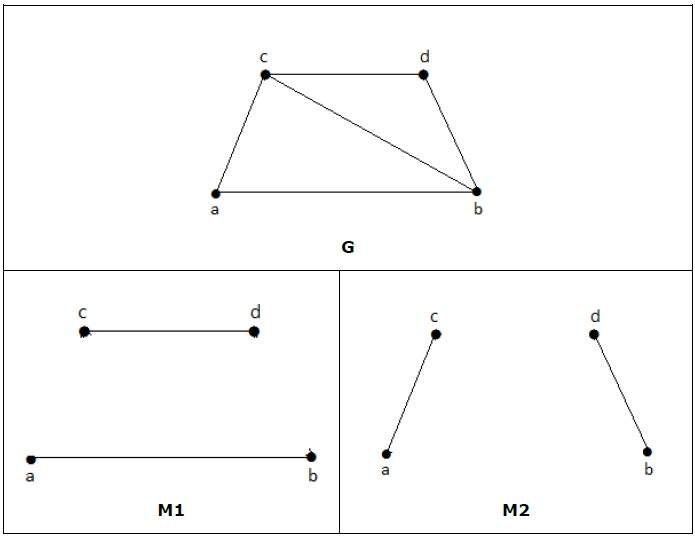
\includegraphics[width=.60\textwidth]{perfect.png}
\caption{$M_{1}$ e $M_{2}$ are examples of perfect matching for G}
\end{figure}

\begin{observation}
From the definition above, we deduce:
\begin{enumerate}
\item Every perfect matching of graph is also a maximum matching of graph, because there is no chance of adding one more edge in a perfect matching graph.. As a consequence, it is also maximal.
\item A maximum matching of graph need not be perfect.
\item If a graph G has a perfect matching, then the number of vertices |V(G)| is even. If it were odd, then the last vertex pairs with the other vertex, and finally there remains a single vertex which cannot be paired with any other vertex for which the degree is zero. It clearly violates the perfect matching principle.
\end{enumerate}
\end{observation}

\begin{figure}[htbp]
\begin{minipage}[htbp]{.80\textwidth}
\centering
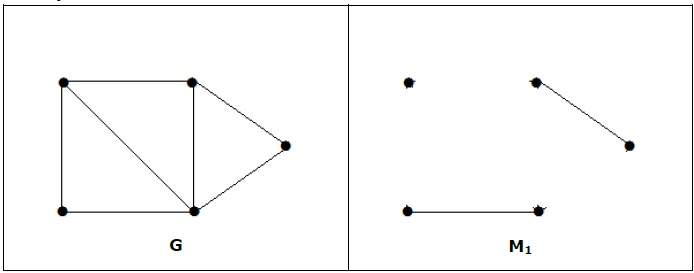
\includegraphics[width=.60\textwidth]{matching1.png}
\caption{The converse of the above statement need not be true. If G has even number of vertices, then $M_{1}$ need not be perfect.}
\end{minipage}
\begin{minipage}[htbp]{.80\textwidth}
\centering
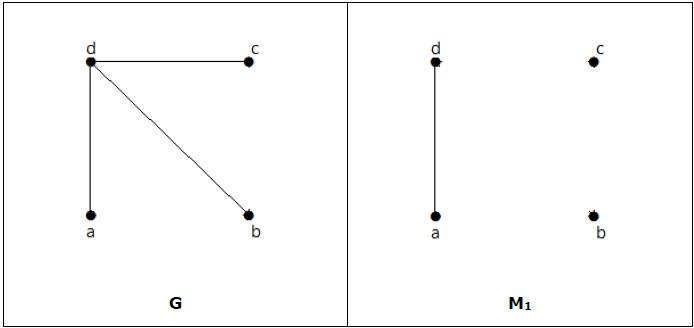
\includegraphics[width=.60\textwidth]{matching2.png}
\caption{It is matching, but it is not a perfect match, even though it has even number of vertices}
\end{minipage}
%\medskip per saltare riga
\end{figure}

%% 1.3
\section{Some examples of Perfect Matching}
To model some problems about Perfect Matching, you often use bipartite graphs. Let $G = (V,E)$ be a bipartite graph with bipartition $\left \{A,B \right \}$, i.e $V = A \cup B$ and $A \cap B = \emptyset$ and all edges link vertices from A to B. Our aim is to find a matching M in G with as many edges as possible.

\begin{definition}
A path in G which starts in A at an unmatched vertex and then contains, alternately, edges from E $\smallsetminus M$ and from M is called alternating path with respect to M.\\
An alternating path P that ends in an unmatched vertex B is called an augmenting path.
\end{definition}
To solve some problems about combinations, you use concepts about graph theory. In this section, we are going to deal with some simple examples of perfect matching and how to solve them. For this reason, we state a very useful result

\begin{theorem}[Hall, 1935]
A bipartite graph G admits a matching A if and only if
\begin{equation*}
|N(S)| \ge |S| \qquad \forall S \subseteq A
\end{equation*}
\end{theorem}
\begin{proof}
See $[1]$.
\end{proof}

\begin{example}
Suppose I have 6 gifts (labeled 1,2,3,4,5,6) to give to 5 friends (Alice, Bob, Charles, Dot, Edward). Can i distribute one gift to each person so that everyone gets something they wish? Certainly, this depends on the preferences of my friends. If none of them like any of my gifts, then I am out of luck. But even if they all like some gifts, I may still not be able to give them out satisfactiorily. For instance, if none of them like gifts 5 or 6, then I will have only 4 gifts to give to my 5 friends and so the problem admits no solutions. We exclude these two particular cases.

\begin{figure}[htbp]
\centering
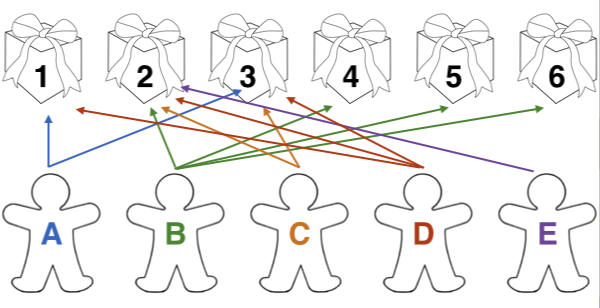
\includegraphics[width=.60\textwidth]{bambini.png}
\caption{Can every child receive the gift he/she prefers?}
\end{figure}

We can model this situation as a graph partioned into two sets: the set of the gifts and the set of the friends. By definition, it is clear that the graph is bipartite. An edge is associated to each child which denotes the preferences about the gifts (for instance, Alice wishes gift 1 or 3 and so on). Let's check if it satisfies or not Hall's theorem: we consider a subset $X = \left \{ A,C,D,E \right \}$, hence $|X| = 4$ and as a consequence $N(X) = \left \{ 1,2,3 \right \}$, so $|X| = 3$. From this, we deduce that $|X| \ge |N(X)|$, thus Hall's condition has been violated and so there no exists a matching. In other words, it is not possible to distribute to everyone the desired gift.
\end{example}

Another example is the vertex cover problem.
\begin{definition}
Let $G = (V,E)$ be a graph. A vertex cover of G is a subset $U \subseteq V$ such that every edge $e \in E$ is incident to a vertex $v \in U$.
\end{definition}
This means that every vertex in the graph is touching at least one edge. Vertex cover is a topic in graph theory that has applications in matching problems and optimization problems. A vertex cover might be a good approach to a problem where all of the edges in a graph need to be included in the solution. In particular, you ask to find minimum vertex cover. 

\begin{figure}[htbp]
\begin{minipage}[htbp]{.80\textwidth}
\centering
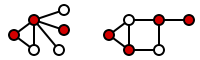
\includegraphics[width=.60\textwidth]{cover.png}
\caption{Examples of vertex cover}
\end{minipage}
\begin{minipage}[htbp]{.80\textwidth}
\centering
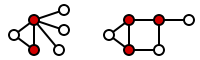
\includegraphics[width=.60\textwidth]{cover1.png}
\caption{Examples of minimum vertex cover}
\end{minipage}
%\medskip per saltare riga
\end{figure}

\begin{observation}
\begin{itemize}
We just report some properties of Vertex Cover:
\item The set of all vertices is a vertex cover;
\item Endpoints of a maximal matching form a vertex cover;
\item The complete bipartite graph $K_{m,n}$ has a minimum vertex cover given by $min\left \{m,n \right \}$.
\end{itemize}
\end{observation}

The following result establishes a link between vertex cover and perfect matching. In particular
\begin{theorem}[K\"onig, 1931]
In a bipartite graph G, the number of edges in a maximum matching is equal to the number of vertices in a minimum vertex cover.
\end{theorem}
\begin{proof}
See $[1]$.
\end{proof}

%\begin{ese}

%You have an art gallery with many hallways and turns. Your gallery is displaying very valuable paintings, and you want to keep them secure. You are planning to install security cameras in each hallway so that the cameras have every painting in view. If there is a security camera in a hallway, it can see every painting in the hallway. If there is a camera in the corner where two hallways meet (the turn), it can view paintings in both hallways. We can model this system as a graph where the nodes represent the places where the hallways cross each other or when a hallway becomes a dead end, and the edges are the hallways. Our aim is to find "strategic" places where to install security cameras.\\
%The easiest solution is to put them in every node: by definition, it is a vertex cover since all edges must be connected to at least one vertex. Doing so, we do not have any risk. However, we suppose that every security camera has a cost, so we want to find the minimum number possible of cameras in order to minimize also the costs. With this assumption, we want to solve the minimum vertex cover problem.\\
%The following picture shows some possible solutions:

\begin{figure}[htbp]
\centering
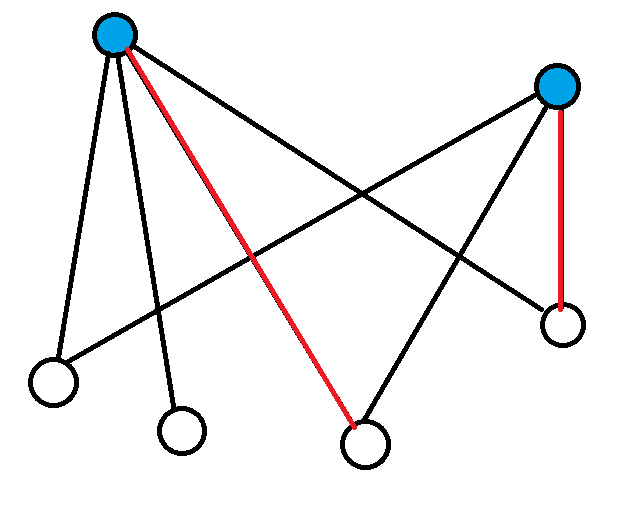
\includegraphics[width=.60\textwidth]{Pm.png}
\caption{Example of application of K\"onig Theorem: red vertices are the minimum vertex cover and blue edges are the maximum matching}
\end{figure}
%\end{ese}


\chapter{Algorithm}
Before explaining all details about the algorithm we developed, we need to introduce some theoretical concept. \\

Consider a graph $G = (V, E)$, defined as a couple of sets: $V$ for vertices, $E$ for edges; $\delta_{G}(S)$ (or $\delta(S)$) is the set of those edges in $E$ with precisely one end-vertex in $S$, subset of $V$. We define a \emph{graft} $(G,T)$ as a connected graph $G$\footnote{A graph $G = (V,E)$ is said \emph{connected} if, for all pairs $(u,v) \in V$ there exists a path between them. A maximal connected subgraph of an undirected graph is said \emph{connected component} of the graph.} in which an even number of vertices $T \subseteq V$ have been distinguished as \emph{odd}. The \emph{T-parity} of a set of vertices $S \subseteq V$ is the parity of $|S \cap T|$. When $S \subseteq V$ is $T$-odd then $\delta(S)$ is a \emph{T-odd cut} or \emph{T-cut}. \\
  
 In order to make a complete description of the algorithm developed, consider the following concept: the \textbf{Gomory-Hu tree}\footnote{Recall that an acyclic graph is a \emph{forest} and a connected forest is a \textbf{tree}} of an undirected graph, i.e. a graph without orientation, is a weighted tree that represents the minimum $\{s,t\}$-cuts for all $\{s,t\}$ pairs in the graph. The Gomory-Hu tree can be constructed in $|V| - 1$ maximum flow computations.
 
 \begin{definition}
 Let $G = ((V_G, E_G), c)$ be an undirected graph with $c(u,v)$ being the capacity of the edge $(u,v)$ respectively. Denote the minimum capacity of an $\{s,t\}$-cut by $\lambda_{s,t}$ for each $\{s,t\} \in V_G$. Let $T = (V_T, E_T)$ be a tree with $V_T = V_G$, denote the set of edges in an $\{s,t\}$ path by $P_{s,t}$ for each $\{s,t\} \in V_T$. Then $T$ is said to be a \textbf{Gomory-Hu tree} of $G$ if
 \[
 \lambda_{s,t} = \min_{e \in P_{s,t}} c(S_e, T_e) \quad \text{for all} \quad \{s,t\} \in V_{G},
 \]
 where
 \begin{enumerate}
 \item $S_e$ and $T_e$ are the two connected components of $T \setminus \{e\}$ in the sense that $(S_e, T_e)$ forms a $s,t$-cut in G. \\
 \item $c(S_e, T_e)$ is the capacity cut in G.
 \end{enumerate}
 \end{definition}
Let $(G,T)$ be a graft and $c: E \to \R_+$ be a \emph{cost} function. A minimum $T$-cut for $(G,T,c)$ is a $T$-cut $\delta(X)$ of $(G,T)$ for which:
\[
c(\delta(X)) = \lambda_{G,T} = \min\{c(\delta(S)): \delta(S)\quad \text{is a $T$-cut of}\quad(G,T) \}
\]
where the cost $c(F)$ of a set $F$ of edges is defined as $\sum_{e \in F} c(e)$.
In particular, we recall some basic facts about submodularity and uncrossing. The complement in $V$ of $S \subseteq V$ is denoted by $\bar{S} = V \setminus S$. \emph{Switching} $S$ means replacing $S$ by $\bar{S}$. For example, if $S = X$, then after switching $S$ we obtain that $S = \bar{X}$ and $\bar{S} = X$. \\
Let $(G, T)$ be a graft and $S \subseteq V$ a set of nodes. 

\begin{observation}
Switching S does not change the $T$-parity of a $S$ (nor  $\delta(S)$), since $|S \cap T|$ and $|\bar{S} \cap T|$ have the same parity since $|T|$ is even.
\end{observation}

\begin{proposition}
Let (G,T) be a graft and $S, X \subseteq V$. Then we have: 
\begin{enumerate}
\item Switching S change the $T$-parity of $S \cap X$ if and only if $X$ is T-odd.\\
\item $S \cap X$ and $S \cup X$ have the same $T$-parity if and only if $S$ and X have the same T-parity. \\
\item Switching S changes the T-parity of $S \cup X$ if and only if X is T-odd.
\end{enumerate}
\end{proposition}

\begin{proof}
Note that $|(S \cap X) \cap T| = |S \cap (X \cap T)|$ whose parity is affected by switching $S$ if and only if $|X \cap T|$ is odd, that is, if and only if $X$ is $T$-odd. This gives $(1)$. To obtain $(2)$ note that $|(S \cap X) \cap T| + |(S \cup X) \cap T| = |S \cap T| + |X \cap T|$. Finally, $(3)$ is a consequence of $(1)$ and $(2)$.
\end{proof}

The following lemma expresses a property of cuts known as \emph{submodularity}.
\begin{lemma}
Let G be a graph with cost function $c: E \longmapsto \R_+$. Let $S_{1}, S_{2} \subseteq V$.
\begin{equation}
c(\delta(S_{1} \cap S_{2})) + c(\delta(S_{1} \cup S_{2})) \leq c(\delta(S_1)) + c(\delta(S_2))
\end{equation}
\end{lemma}

\begin{proof}
We claim that each edge $uv$ contributes to the right at least as to the left side of (2.1). By Proposition 2.2, if $S_1 \cap S_2$ have different $\{u,v\}$-parities, so do $S_1$ and $S_2$. Hence, had our claim to be false, then both $S_1 \cap S_2$ and $S_1 \cup S_2$ would be $\{u,v\}$-odd. Assume w.l.o.g. that $u \in S_1 \cup S_2$ and $u \notin S_1 \cup S_2$. Then, $u \in S_1, S_2$ and $u \notin S_1, S_2$
\end{proof}

If $S \cap X \neq \O$ for every possible switching of $S$ and $X$, then $S$ and $X$ are said to \emph{cross}. All what we will need about cut functions is that they obey to the following lemma. 

\begin{lemma}
Let $T_{1}, T_{2}$ be even cardinality subsets of V. Let $\delta(S_1)$ be a minimum $T_1$-cut and assume that $S_1$ is $T_2$-even. Then there exists a minimum $T_2$-cut $\delta(S_2)$ such that $S_1$ and $S_2$ do not cross.
\end{lemma}

\begin{proof}
Let $\delta(X)$ be a minimum $T_2$-cut. We remark that, by Proposition 2.2, switching $S_1$ changes the $T_2$-parity of $S_1 \cup X$ whereas switching $X$ changes the $T_1$-parity of $S_1 \cap X$ leaving the $T_2$-parity of $S_1 \cup X$ unaffected. Therefore, by possibly switching $S_1$, we can assume that $S_1 \cup X$ is $T_2$-odd. Afterwards, by possibly switching $X$, we can assume that $S_1 \cap X$ is $T_1$-odd without affecting the $T_2$-parity of $S_1 \cup X$. 
At this point, $c(\delta(S_1 \cup X)) \ge c(\delta(S_1))$ since $\delta(S_1)$ is a minimum $T_1$-cut. By sub-modularity, $c(\delta(S_1 \cup X)) = c(\delta(X))$. Thus, $\delta(S_1 \cup X)$ is a minimum $T_2$-cut. And clearly, $S_1$ and $S_1 \cup X$ do no cross. 
\end{proof}

\section{Minimum $T$-cuts: a simple algorithm}
Now, we will present an algorithm for $T$-cut. Consider a graft $(G,T)$ and a $T$-even set $S \subseteq V$, denoted by $G_S$ the graph obtained from $G$ by identifying all nodes in $S$ into a single node and letting $T_S := T \setminus S$. Note that $(G_S, T_S)$ is a graft. When $S = \{ s, t \} \subseteq T$ then we rely on a shorter notation $G_{s,t} = G_{\{s,t\}}$ and $T_{s,t} = T_{\{s,t\}}$. \\
Since node identification does not affect the edge set of a graph, a cost function $c$ for $G$ is also a cost function for $G_S$ and $G_{s,t}$.
Then, we show four steps to compute $\lambda_{G,T}$:\\

\texttt{MinT-cut(G,T,c)}
\begin{enumerate}
\item if $T = \O$ then return $\infty$, that means $(G,T)$ does not contains any $T$-cut;\\
\item let $s$ and $t$ be any two different nodes in $T$; \\
\item let $\delta(S)$ be a minimum $\{s,t\}$-cut; \\
\item if $S$ is $T$-odd then return $\min( c(\delta(S)), \texttt{MinT-cut($G_{s,t}, T_{s,t}$, c)})$; otherwise return $\min(\texttt{MinT-cut($G_{S}, T_{S}$, c)}; \texttt{MinT-cut($G_{\bar{S}}, T_{\bar{S}}$, c)})$
\end{enumerate}

\section{Correctness}
For a given $(G,T,c)$, let $s$ and $t$ be any two different nodes in $T$ and let $\delta(S)$ be a minimum $\{s,t\}$-cut. The correctness of the above procedure relies on the following two lemmas:
\begin{lemma}
If $\delta(S)$ is T-odd, then $\lambda_{G,T} = \min(c(\delta(S)), \lambda_{G_{s,t}, T_{s,t}})$.
\end{lemma}

\begin{proof}
Indeed, the $T_{s,t}$-cuts of $G_{s,t}$ are precisely the $T$-cuts of $G$ that are not $\{s,t\}$-odd.
\end{proof}

\begin{lemma}
If $\delta(S)$ is T-even, then $\lambda_{G,T} = \min( \lambda_{G_{S}, T_{S}}, \lambda_{G_{\bar{S}}, T_{\bar{S}}})$.
\end{lemma}

\begin{proof}
First note that every $T_S$-cut in $(G_S, T_S)$ and every $T_{\bar{S}}$-cut in $(G_{\bar{S}},T_{\bar{S}})$ is also a $T$-cut in $(G,T)$. This implies $\lambda_{G,T} \le \min( \lambda_{G_{S}, T_{S}}, \lambda_{G_{\bar{S}}, T_{\bar{S}}})$. 
For the converse, let $\delta(X)$ be any minimum $T$-cut for $(G,T,c)$. By Lemma 2.4, we can assume that $S$ and $X$ do not cross. This means that the edge set $\delta_{G}(X)$ is either a $T_S$-cut in $G_S$ or a $T_{\bar{S}}$-cut in $G_{\bar{S}}$.
\end{proof}

\section{Computing optimal $T$-parings}
Let $(G,T)$ be a graft with cost function $c: E \longmapsto \R_+$. A \emph{T-pairing} is a partition of $T$ into pairs. The value of the $T$-pairing $\mathcal{P}$ is defined as: 
\[
val_G (\mathcal{P}) = \min_{\{u,v\} \in \mathcal{P}} \lambda_{G}(u,v) 
\]
where $\lambda_G (u,v)$ denotes the cost of a minimum $\{u,v\}$-cut, Let $\mathcal{P}$ be any $T$-pairing and $\delta(S)$ be any $T$-cut. Since $\delta(S)$ is $T$-odd, $\mathcal{P}$ contains a pair $\{u,v\}$ such that $\delta(S)$ is $\{u,v\}$-odd. Therefore, $c(\delta(S)) \ge \lambda_G (u,v) \ge val_G (\mathcal{P})$ and the value of $\mathcal{P}$ is a lower bound on $\lambda_{G,T}$.\\
In this section, we show that the algorithm \emph{MinT-cut} actually finds a $T$-pairing of value $\lambda_{G,T}$. Indeed, consider a single iteration of the algorithm. Let $s$ and $t$ be two odd nodes. Let $\delta(S)$ be a minimum $\{s,t\}$-cut. 

\begin{lemma}
Let $\delta(S)$ be a minimum $\{s,t\}$-cut in $(G,c)$. Then we have: 
\[
\lambda_G (u,v) \ge \min(c(\delta(S)), \lambda_{G_{s,t}}(u,v)) \qquad \forall u,v \in V(G) \setminus \{s,t\}
\]
\end{lemma}

\begin{proof}
Indeed, the $\{u,v\}$-cuts of $G_{s,t}$ are exactly the $\{u,v\}$-cuts of $G$ that are not $\{s,t\}$-odd.
\end{proof}

\begin{lemma}
Let $\delta(S)$ be a minimum $\{s,t\}$-cut in $(G,c)$. Then we have: 
\[
\lambda_G (u,v) = \lambda_{G_{s}} (u,v) \qquad \forall u,v \in V(G) \setminus S
\]
\end{lemma}

\begin{proof}
Let $u$ and $v$ be two any nodes in $V(G) \setminus S$. Obviously $\lambda_G (u,v) \le \lambda_{G_{s}} (u,v)$. For the converse, let $\delta(X)$ be any minimum $\{u,v\}$-cut in $G$. By Lemma 2.4, we can assume that $S$ and $X$ do not cross. Then, the edge set $\delta_{G}(X)$ is a $\{u,v\}$-cut in $G_S$ and $\lambda_G (u,v) = \lambda_{G_{s}} (u,v)$.
\end{proof}

Each iteration of the algorithm contemplates two possibilities: 
\begin{enumerate}
\item \textbf{Case 1}: $\delta(S)$ is $T$-odd. By Lemma 2.5, $\lambda_{G,T} = \min\{c(\delta(S)), \lambda_{G_{s,t},T_{s,t}}\}$. By Lemma 2.7, if $\mathcal{P'}$ is a $T_{s,t}$-pairing with $val_{G_{s,t}}(\mathcal{P'}) = \lambda_{G_{s,t},T_{s,t}}$, then $\mathcal{P} = \mathcal{P'} \cup \{s,t\}$ is a $T$-pairing with $val_{G} (\mathcal{P}) \ge \min(c(\delta(S)), val(\mathcal{P'})) = \min(c(\delta(S)), \lambda_{G_{s,t},T_{s,t}}) = \lambda_{G,T}$. \\
\item \textbf{Case 2}: if $\delta(S)$ is $T$-even. By Lemma 2.6, $\lambda_{G,T} = \min\ \lambda_{G_{S},T_{S}}, \lambda_{G_{\bar{S}},T_{\bar{S}}}\}$. By Lemma 2.8, if $\mathcal{P_S}$ is a $T_{S}$-pairing with $val_{G_{S}} (\mathcal{P_S}) = \lambda_{G_{S},T_{S}}$ and $\mathcal{P_{\bar{S}}}$ is a $T_{\bar{S}}$-pairing with $val_{G_{\bar{S}}} (\mathcal{P_{\bar{S}}}) = \lambda_{G_{\bar{S}},T_{\bar{S}}}$ then $\mathcal{P} = \mathcal{P_S} \cup \mathcal{P_{\bar{S}}}$ is a $T$-pairing with $val_{G} (\mathcal{P}) \ge \min(val(\mathcal{P_S}), val(\mathcal{P_{\bar{S}}})) = \min(\lambda_{G_{S},T_{S}}\lambda_{G_{\bar{S}},T_{\bar{S}}}) = \lambda_{G,T}$.
\end{enumerate}  

The following results summarize this section. 

\begin{theorem}
For every $(G,T,c)$ the maximum value of a $T$-pairing equals the minimum cost of a T-cut.
\end{theorem}

\begin{theorem}
For every node u in T there exists a node $v \in T \setminus \{u\}$ such that $\{u,v\}$ is useful.
\end{theorem}

\begin{proof}
Apply algorithm \emph{MinT-cut} to $(G,T,c)$. At each recursion, keep choosing $s = u$ until the minimum $\{s,t\}$-cut $\delta(S)$ is $T$-odd. By Lemma 2.8, $\{u,v\}$ is useful w.r.t. $(G,T,c)$.
\end{proof}

\section{Algorithm}
We have developed an algorithm on Python using both Gurobi and Python languages. It can be run using Spyder\footnote{It is in Anaconda.}(full code is in Appendix A). In what follows, we analyze the main aspects of the algorithm. It is composed of two parts: 
\begin{enumerate}
\item In the first part, we gave four important functions: \texttt{Contraction}, \texttt{minCutValue}, \texttt{findsubsets} and \texttt{minCutEdges};\\
\item After that,  we developed the model (constraint and objective function). The final \texttt{while} cycle optimize the model. 
\end{enumerate}

We start analyzing the second part of the code. First, we create the variables: we define a lower bound at zero and consider them continuous as type. At the beginning, we defined them as binary variable, but in this way we always found an integer solution. So in order to solve a real problem (i.e. non integer solution), we have decided to change the variables type as continuous. In this case, at first we obtain a non-integer solution. 
Then we add the objective function: 
\[
\min \sum_{ij} \texttt{edges} \cdot \texttt{var}
\]
that minimizes the sum of all products between the continuous variable \texttt{var} and \texttt{edges} which represents the cost value of the considered edge. The only constraint we consider: the sum of all edges entering in a certain vertex must be 1. \\
After looking for edges incident to a vertex $i$ and after building up the constraint we explained before, we define the optimization model. We iteratively make the code looking for integer solution thanks to a while-cycle. This means that, in the cycle, it optimizes the model, then it finds the value of minimal odd cut and checks if this value is less or greater than 1. \\
If the minimal odd cut is less than 1, it finds the edges of the minimal odd cut and adds a constraint, that is the sum of the variables associated to the edges of the minimal cut have to be greater or equal to 1.  And so on, until it finds an integer solution. \\

In the first part of the code, we import firstly the useful modules we need to develop the optimization model. This part is based on finding minimum $T$-cut.
We define a function for contraction, which at the end creates a minor of $G$. Then, the function \texttt{minCutValue(graph, T)} finds the value of minimum odd cut  of a given graph; \texttt{T} is a datum used during the recursion: it must be initially set equal to '\texttt{vertices}'. The third function we define is \texttt{findsubset}, which finds all subsets of a fixed cardinality of a given set. Given a graph and the value of one of its minimum odd cuts, we construct a function which finds the edges of the minimum odd cut \texttt{minCutEdges}.   \\

In another file Python we have considered some graphs on which test the algorithm, such as Petersen graph, TSP problem, an unfeasible graph (i.e. a graph which has not a perfect matching) and $K(5)$ graph which are described in Appendix B. 


\chapter{Conclusion}
Despite the advantages of the algorithm presented, the code can be improved. For example, the following changes can be made:
\begin{itemize}
\item the dictionaries (.keys inside the code) could be used for the vertices and not for the arcs, but in this case we should solve the problem of the weights to assign to the arcs;
\item the examples were placed in a separate python file and it could be able to structure it as a text file and recall it in the python matching file;
\end {itemize}

The initial idea was to use the Call-Back functions, i.e. to use it within the while loop as in the case of the TSP (Traveler Salesman Problem). In this case, however, the Call-Back functions could not be used because Gurobi does not allow the user to use the value of the variables except in the MIP phase, i.e. in a phase of the process in which there are only whole values of the solutions , but the problem that you want to get around with this algorithm is to use only whole values of the solutions.

So we came to a contradiction and we had to discard the idea of using Call-Back within the code.

In conclusion, the algorithm can be improved through the resolution of some problems and the problem of using a certain type of functions within the code due to program restrictions has been circumvented.

\appendix
\chapter{Perfect-Matching Code}
\begin{verbatim}
@author: Alessandro Zeggiotti
# -------------------------------------------------------------------
# USEFUL MODULES

import math
import random
from gurobipy import *

import networkx as nx
import itertools

# Matching_examples.py contains some useful examples to test this script
# QUESTION: Is "import" the best way to run an external script?
from Matching_examples import *

# -------------------------------------------------------------------
# FUNCTIONS DEFINITION

# Given a graph, this function idefintifies a set of nodes into a single vertex

def Contraction(graph, nodes):
    V = set()
    for i,j in graph:
        V = V.union({i})
        V = V.union({j})
    new_vertex = max(V) + 1
    # Create a minor of the graph
    minor = {}
    for i,j in graph.keys():
        if i in nodes and j in nodes:
            pass
        elif i in nodes and (j,new_vertex) not in minor.keys():
            minor[j,new_vertex] = graph[i,j]
        elif i in nodes:
            minor[j,new_vertex] += graph[i,j]
        elif j in nodes and (i,new_vertex) not in minor.keys():
            minor[i,new_vertex] = graph[i,j]
        elif j in nodes:
            minor[i,new_vertex] += graph[i,j]
        else:
            minor[i,j] = graph[i,j]
    return minor

# Given a graph, this function finds the value of a minimum odd cut
# T is a datum used during the recursion: 
#it must be initially set equal to "vertices"

def minCutValue(graph, T):
    # Base step
    if T == set():
        return float('inf')
    # Create the graph using the module NETWORKX
    G = nx.DiGraph()
    for (i,j) in graph.keys():
        G.add_edge(i, j, capacity = graph[i,j])
        G.add_edge(j, i, capacity = graph[i,j])
    # Let s and t be two random nodes in T
    s = min(T)
    t = max(T)
    # NETWORKX contains a function that allows to find the minimum s-t cut
    # This function is based on Ford-Fulkerson algorithm
    cut_value, partition = nx.minimum_cut(G,s,t)
    S, S_bar = partition
    if len(S.intersection(T)) % 2 == 1: # if S is T-odd: ...
        return min(cut_value,
                   minCutValue(Contraction(graph, {s,t}), T - {s,t}))
    else:
        return min(minCutValue(Contraction(graph, S), T - S),
                   minCutValue(Contraction(graph, S_bar), T - S_bar))

# Given a set, this function finds all its subsets of a fixed cardinality

def findsubsets(S,m):
    # From ITERTOOLS module
    return set(itertools.combinations(S, m))

# Given a graph and the value of a minimum odd cut, 
# this function finds a minimum odd cut

def minCutEdges(graph, cut_value):
    for cardinality in range(1,n,2):
        subsets = findsubsets(vertices, cardinality) 
        # "vertices" is global variable
        for S in subsets:
            # Create the cut
            dS = {}
            for i,j in graph.keys():
                if i in S and j not in S:
                    dS[i,j] = graph[i,j]
                if i not in S and j in S:
                    dS[i,j] = graph[i,j]
            dS_value = sum(dS.values())
            if dS_value == cut_value:
                return dS
    print('No odd cut of value %g has been found' % cut_value)
    return None

# -------------------------------------------------------------------
# MODEL DEFINITION

m = Model()
# Suppress the standard output, it would be invoked too many times
m.setParam('OutputFlag', 0)

# Create the variables
vars = {}
for (i,j) in edges.keys():
   vars[i,j] = m.addVar(lb=0, vtype=GRB.CONTINUOUS, name='e[%d,%d]'%(i,j))

# To create the model data structure only once, after variables creation
m.update()

# Add the objective function
m.setObjective(sum(vars[i,j]*edges[i,j] for i,j in edges.keys()), GRB.MINIMIZE)

# Add degree-1 constraint
for i in vertices:
    # Look for the edges incident to i
    neighbors = []
    for j in vertices:
        if (i,j) in edges.keys():
            neighbors.append((i,j))
        elif (j,i) in edges.keys():
            neighbors.append((j,i))
    m.addConstr(sum(vars[i,j] for i,j in neighbors) == 1)

# -------------------------------------------------------------------
# MODEL OPTIMIZATION

linked = set()
for edge in edges.keys():
    linked = linked.union(set(edge))

# Check the presence of isolated vertices
if vertices != linked:
    print(str(vertices - linked) + ' is a set of isolated vertices!')

# Check the parity of the graph
elif n % 2 == 1:
    print('The graph is odd!')

else:
    # Now we are sure that the graph admits a solution
    while True:
        # Solve the problem
        m.optimize()
        print('\n--------------------------------------------------------\n')
        solution = m.getAttr('x', vars)
        selected = [(i,j) for i,j in solution.keys() if solution[i,j] != 0]
        print('New incumbent solution:\n')
        for i,j in selected:
            print('    ' + str((i,j)) + ' : ' + str(solution[i,j]))
        print('\nObjective function: %g' % m.objVal)
        print('Checking the presence of rationals...')
        # Find the value of a minimum odd cut
        cut_value = minCutValue(solution, vertices)
        if cut_value < 1:
            # Find the edges of a minimum odd cut
            cut_edges = minCutEdges(solution, cut_value)
            # Add a constraint
            m.addConstr(sum(vars[i,j] for (i,j) in cut_edges.keys()) >= 1)
            print('Minimum odd cut: %g' % cut_value)
            print('Related edges:\n')
            for i,j in cut_edges.keys():
                print('    ' + str((i,j)) + ' : ' + str(cut_edges[i,j]))
            print('\nNew constraint added...')
        else:
            print('This is a feasible solution!')
            break
\end{verbatim}
\chapter{Perfect-Matching Code Examples}
\begin{verbatim}
@author: Alessandro Zeggiotti
"""

# Create vertices and edges for our example
# The user can choose one among the four following graphs
print('\n1 --> TSP problem')
print('2 --> Petersen graph')
print('3 --> Unfeasible graph')
print('4 --> K(5)')
choice = int(input('Choose your favourite example: '))

if choice == 1:
    vertices = {0,1,2,3,4,5}
    edges = {
        (0,1): 5,
        (0,2): 5,
        (0,3): 4,
        (1,4): 2,
        (1,5): 3,
        (2,3): 3,
        (2,5): 8,
        (3,4): 4,
        (4,5): 4}
elif choice == 2:
    vertices = {0,1,2,3,4,5,6,7,8,9}
    edges = {
        (0,1): 1,
        (0,4): 1,
        (0,5): 1,
        (1,2): 1,
        (1,6): 1,
        (2,3): 1,
        (2,7): 1,
        (3,4): 1,
        (3,8): 1,
        (4,9): 1,
        (5,7): 1,
        (5,8): 1,
        (6,8): 1,
        (6,9): 1,
        (7,9): 1}
elif choice == 3:
    vertices = {0,1,2,3}
    edges = {
        (0,2): 1,
        (0,3): 1,
        (2,3): 1}
else:
    vertices = {0,1,2,3,4}
    edges = {
        (0,1): 1,
        (0,2): 1,
        (0,3): 1,
        (0,4): 1,
        (1,2): 1,
        (1,3): 1,
        (1,4): 1,
        (2,3): 1,
        (2,4): 1,
        (3,4): 1}

n = len(vertices)


\end{verbatim}

\begin{thebibliography}{90}        
%\begin{enumerate}[{[K1]}]
\bibitem{K1} Reinhard Diestel, "Graph Theory", Electionic Edition 2005
\bibitem{K2} John M. Harris, Jeffry L. Hirst, Michael J.Mossinghoff, "Combinatorics and Graph Theory", Springer Edition 2008
\bibitem{K3} Romeo Rizzi, "A Simple Minimum T-Cut Algorithm", October 23, 2002
%\end{enumerate}
\end{thebibliography}
\end{document}